%! suppress = LineBreak
%%
%% This is file `sample-sigconf.tex',
%% generated with the docstrip utility.
%%
%% The original source files were:
%%
%% samples.dtx  (with options: `sigconf')
%%
%% IMPORTANT NOTICE:
%%
%% For the copyright see the source file.
%%
%% Any modified versions of this file must be renamed
%% with new filenames distinct from sample-sigconf.tex.
%%
%% For distribution of the original source see the terms
%% for copying and modification in the file samples.dtx.
%%
%% This generated file may be distributed as long as the
%% original source files, as listed above, are part of the
%% same distribution. (The sources need not necessarily be
%% in the same archive or directory.)
%%
%% The first command in your LaTeX source must be the \documentclass command.
\documentclass[sigconf,review,anonymous]{acmart}


% Packages
\usepackage{amsfonts}
\usepackage{amsmath}
\usepackage{graphicx}
\usepackage{hyperref}
\usepackage{float}
\usepackage{pgfplots}
\usepgfplotslibrary{fillbetween}
\usepackage[pdf]{graphviz}
\usepackage{tikz}
\usepackage{natbib}

\usepackage{booktabs}
\usepackage{pifont}
\usepackage{fontspec}
\usepackage{fontawesome}

\newcommand{\wmark}{\textcolor{orange}{\ding{45}}}
\newcommand{\cmark}{\textcolor{green!80!black}{\ding{51}}}
\newcommand{\xmark}{\textcolor{red}{\ding{55}}}

\usepackage{multicol}

% Packages
\usepackage{amsmath}
\usepackage{listings}
\usepackage{fontspec}
\usepackage{xcolor}

\setmonofont{JetBrainsMono}[
  Path=./JetbrainsFontFiles/,
  Extension = .ttf,
  UprightFont=*-Regular,
  BoldFont=*-Bold,
  ItalicFont=*-Italic,
  BoldItalicFont=*-BoldItalic
]

\makeatletter
\def\verbatim@nolig@list{}
\makeatother

\lstdefinelanguage{kotlin}{
  comment=[l]{//},
  commentstyle={\color{gray}\ttfamily},
  emph={delegate, filter, firstOrNull, forEach, it, lazy, mapNotNull, println, repeat, assert, with, head, tail, len, return@},
  numberstyle=\noncopyable,
  emphstyle={\color{OrangeRed}},
  identifierstyle=\color{black},
  keywords={abstract, actual, as, as?, break, by, class, companion, continue, data, do, dynamic, else, enum, expect, false, final, for, fun, get, if, import, in, infix, interface, internal, is, null, object, open, operator, override, package, private, public, return, sealed, set, super, suspend, this, throw, true, try, catch, typealias, val, var, vararg, when, where, while, tailrec, reified},
  keywordstyle={\color{NavyBlue}\bfseries},
  morecomment=[s]{/*}{*/},
  morestring=[b]",
  morestring=[s]{"""*}{*"""},
  ndkeywords={@Deprecated, @JvmField, @JvmName, @JvmOverloads, @JvmStatic, @JvmSynthetic, Array, Byte, Double, Float, Boolean, Int, Integer, Iterable, Long, Runnable, Short, String},
  ndkeywordstyle={\color{BurntOrange}\bfseries},
  sensitive=true,
  stringstyle={\color{ForestGreen}\ttfamily},
  literate={`}{{\char0}}1
}

%% NOTE that a single column version may be required for
%% submission and peer review. This can be done by changing
%% the \doucmentclass[...]{acmart} in this template to
%% \documentclass[manuscript,screen]{acmart}
%%
%% To ensure 100% compatibility, please check the white list of
%% approved LaTeX packages to be used with the Master Article Template at
%% https://www.acm.org/publications/taps/whitelist-of-latex-packages
%% before creating your document. The white list page provides
%% information on how to submit additional LaTeX packages for
%% review and adoption.
%% Fonts used in the template cannot be substituted; margin
%% adjustments are not allowed.
%%
%%
%% \BibTeX command to typeset BibTeX logo in the docs
\AtBeginDocument{%
  \providecommand\BibTeX{{%
    \normalfont B\kern-0.5em{\scshape i\kern-0.25em b}\kern-0.8em\TeX}}}

%% Rights management information.  This information is sent to you
%% when you complete the rights form.  These commands have SAMPLE
%% values in them; it is your responsibility as an author to replace
%% the commands and values with those provided to you when you
%% complete the rights form.
\setcopyright{acmcopyright}
\copyrightyear{2022}
\acmYear{2022}
\acmDOI{10.1145/1122445.1122456}

%% These commands are for a PROCEEDINGS abstract or paper.


\acmConference[ICSE 2022]{The 44th International Conference on Software Engineering}{May 21–29, 2022}{Pittsburgh, PA, USA}


\newcommand{\seqWord}{Seq \langle Word \rangle}
\newcommand{\distSeqWord}{Dist\langle \seqWord  \rangle}

%%
%% Submission ID.
%% Use this when submitting an article to a sponsored event. You'll
%% receive a unique submission ID from the organizers
%% of the event, and this ID should be used as the parameter to this command.
%%\acmSubmissionID{123-A56-BU3}

%%
%% The majority of ACM publications use numbered citations and
%% references.  The command \citestyle{authoryear} switches to the
%% "author year" style.
%%
%% If you are preparing content for an event
%% sponsored by ACM SIGGRAPH, you must use the "author year" style of
%% citations and references.
%% Uncommenting
%% the next command will enable that style.
%%\citestyle{acmauthoryear}

%%
%% end of the preamble, start of the body of the document source.
\begin{document}

%%
%% The "title" command has an optional parameter,
%% allowing the author to define a "short title" to be used in page headers.
  \title{How sensitive is neural code completion to syntactic variance?}
% \title{Code Transformations
% Neural language models
% Interpretability
% Reliability/Robustness
% Comprehension/Understanding

% }

% \title{An empirical study of source code transformations on the robustness of neural language models}
%%
%% The "author" command and its associated commands are used to define
%% the authors and their affiliations.
%% Of note is the shared affiliation of the first two authors, and the
%% "authornote" and "authornotemark" commands
%% used to denote shared contribution to the research.
  \author{Breandan Considine, Xujie Si, Jin L.C. Guo}
  \email{breandan.considine@mail.mcgill.ca, {xsi, jguo}@cs.mcgill.ca}
  \affiliation{%
    \institution{McGill University}
  }

%%
%% By default, the full list of authors will be used in the page
%% headers. Often, this list is too long, and will overlap
%% other information printed in the page headers. This command allows
%% the author to define a more concise list
%% of authors' names for this purpose.
% \renewcommand{\shortauthors}{Trovato and Tobin, et al.}

%%
%% The abstract is a short summary of the work to be presented in the
%% article.
  \begin{abstract}
    Neural language models hold great promise as tools for computer-aided programming, but questions still remain as to their reliability and the consequences of overreliance on those tools. In the domain of natural language, prior work has revealed these models can be sensitive to naturally-occurring variance and malfunction in unpredictable ways. A closer examination of neural language models is thus needed to understand their behavior on programming-related tasks. In this work, we develop a methodology for systematically evaluating neural language models using simple source code transformations such as synonymous renaming, intermediate logging, and independent statement reordering. Applying these transformations to natural code snippets, we evaluate three state-of-the-art models, CodeBERT, GraphCodeBERT and RobertA-Java, which exhibit varying degrees of robustness. Our approach is implemented and released as a modular and extensible toolkit for evaluating the performance of neural code completion models.

    % complacency can lead to increased reviewer burden or more serious technical debt. While trade secrecy may prevent third-party inspection of pretrained models, users would still like some assurance of the model's robustness to naturally-occurring variance.

    % What is the key message?
    %   - Different types of SCTs
    %.  - Different types of deep learning models (e.g. RNNs, transformers)
    %   - Different types of Evaluation tasks (e.g. code completion)
    %.  - Different measures of robustness (e.g. latent space, predictions)
    %
  \end{abstract}

  \maketitle

  \section{Introduction}\label{sec:introduction}

  Statistical language models play an increasingly synergetic role in software development, most prominently in code completion~\cite{chen2021evaluating}. Yet from a user's perspective, the behavior of these models is opaque: partially completed source code written in an editor is sent to a remote server, which returns a real-time suggestion. This client-server architecture can be seen as a black-box or \textit{extensional} function from a mathematical perspective. How can we evaluate the behavior of neural language models in this setting? The role of automated testing becomes apparent.

  First conceived in the software testing literature, metamorphic testing~\cite{chen1995metamorphic} is a concept known in machine learning as \textit{self-supervision}. In settings where labels are scarce but certain \textit{invariants} or \textit{metamorphic relations} are known, one can generate an effectively unlimited amount of data by selecting and recombining synthetic transformations. For example, computer vision models should be invariant to shift, scale and rotation, so given a small dataset of labeled images, we can apply these transformations to obtain far more data for training or evaluation. Do similar invariants exist for source code?

  One would expect code completion models to exhibit invariance to certain refactorings. For example, code completion should be invariant to synonym variable renaming or reordering dataflow-independent statements.

  \section{Method}

  We examine in our work three primary questions. Given a set of (1) source code (2) a set of SCTs, (3) a set of slicing and tokenization methods, how do these factors affect accuracy on the masked code completion task. We sample a the top 100 most-starred Java repositories from GitHub organizations with over 100 forks and between 1 and 10 MB in size. From these, we extract a set of Java methods using the heuristic described in the appendix

  Code transformations... %describe

  How to evaluate source code transformations:

  Comparing different types of transformations

  Combining different transformations or bounds?

  Single vs. multiple transformation benefits (cite testing literature?)

  Code characteristics: different categories of code based on...
  selection: slicing, tokenization..
  language: java, kotlin
  size: method length
  complexity: halstead, cyclometric


%  \section{Prior literature}\label{sec:prior-literature}
%
%  Prior studies of natural langauge in source code have been undertaken ~\citep{weiss2018practical, chirkova2020empirical, chen2021evaluating}, which characterize the families of computational languages that neural langauge models can recognize in practice. Our work builds on this literature from a software engineering standpoint: what kinds of idioms

%  Prior work in the code search literature explores the text-to-code~\citep{husain2019codesearchnet} setting, where queries are typically considered to be a short sequence composed by the user, or code-to-code~\citep{kim2018facoy} setting where the query takes the form of a code snippet. Model performance typically evaluated using mean reciprocal rank (MRR), mean average precision (MAP), normalized discounted cumulative gain (NDCG), precision and recall at top N-results (P/R@N), or similar metrics. Although some~\citep{asyrofi2020ausearch} do incorporate other features from the local document, none however, consider the query in the context of a broader project. The ability to align contextual features from the surrounding project, we argue, is essential to delivering semantically relevant search results.

% {
% \renewcommand{\arraystretch}{1.5}
% \begin{table}[H]
%   \small
%   \begin{tabular}{lllc}
%     Name & Type & Key contribution & Evaluation method \\
%     \hline
%     \href{https://github.com/breandan/gym-fs}{\textsc{Our Work}} & Either-to-Either & Learning to search & Prediction accuracy \\
%     \href{https://core.ac.uk/download/pdf/162022846.pdf#page=7}{\textsc{FaCoY}}~\citep{kim2018facoy} & Code-to-code & Similarity search & MRR \\
%     \href{https://www.jameskoppel.com/files/papers/yogo-preprint.pdf#page=11}{\textsc{Yogo}}~\cite{premtoon2020semantic}     & Code-to-code & Equational reasoning & Case study \\
%     \href{https://arxiv.org/pdf/1909.09436.pdf#page=5}{\textsc{CSNet}}~\citep{husain2019codesearchnet}     & Text-to-code & Big code benchmark & MRR \\
%     \href{https://arxiv.org/pdf/1812.01158.pdf#section.5}{\textsc{Aroma}}~\citep{luan2019aroma}     & Code-to-code & Structural Search& Recall@N \\
%     \href{https://raw.githubusercontent.com/mhilmiasyrofi/AUSearch/master/SANER_2020_AUSearch.pdf}{\textsc{AUSearch}}~\citep{asyrofi2020ausearch}     & Code-to-code & Type resolver & Highlight accuracy \\

%     \href{https://arxiv.org/pdf/1905.03813.pdf#section.4}{\textsc{Cambronero}}~\citep{cambronero2019deep}     & Text-to-code & Semantics & Answered@N \\
%     \href{https://guxd.github.io/papers/deepcs.pdf#section.5}{\textsc{DeepCS}}~\citep{gu2018deep}     & Text-to-code & Deep learning & FRank, *@N, MRR \\
%     \href{https://www.cs.sjtu.edu.cn/~zhonghao/paper/Lancer.pdf}{\textsc{Lancer}}~\citep{zhou2019lancer}     & Code-to-code & BERT embedding & HitRate@k, MRR \\
%   \end{tabular}
%   \caption{\label{tab:ad_comparison} Comparison of existing code search tools.}
% \end{table}
% }

%  Although we draw some inspiration from the duplicate detection literature, their work presumes the code was intentionally duplicated or modified but is essentially identical in form or function. In contrast, our work seeks to help users discover artifacts which predictive of as-yet-incomplete code. By aligning salient features from the surrounding document and project graph, we approximate the notion of semantic similarity, without requring a language-specific parser like some methods~\citep{cambronero2019deep} do, and can more easily adapt to settings where the language and project structure varies.

%   Furthermore, unlike prior work, our work considers the surrounding project and related artifacts. Instead of parsing their contents explicitly, which may be computationally intractable, we allow the agent to construct the graph organically by exploring the filesystem, then extract a query.

  \section{Method}\label{sec:method}



  Do language models learn to recognize patterns in source code? If so, what kinds? A longstanding research area in software engineering tries to extract idioms from large software repositories. Likewise, a longstanding goal of neural program synthesis is compositional generalization. Both currently require designing a feature representation that “selects” for a specific kind of invariance — for example, structural similarity selects for name-invariance, and semantic similarity captures structural invariance.

  In our work, we explore the extent to which recent language models trained on source code learn regularities they were not explicitly designed to represent. We analyze three different language models, and compare their zero-shot generalization on synthetically-generated patterns. We generate code snippet pairs corresponding to manually-designed variance, and measure the effect on various language models. Each model is evaluated on a set of code snippets exposed to synthetic transformations and predicts a masked token.

  Our goal then, is to identify equivariant representations captured by the language model (LM). To do so, we generate program transformations (PTs) and measure vector equivariance in four rewriting categories:

  \begin{enumerate}
    \item Syntactic - can the LM detect syntactically invalid PTs? (e.g. syntax corruption, imbalanced parenthesis)
    \item Structural - can the LM detect syntactically valid, but structurally altered PTs? (e.g. use before declaration, permuted argument order)
    \item Semantic - can the LM detect structurally valid, but semantically altered PTs? (e.g. constant modification, operator substitution and order of operations)
    \item Equivalence - can the LM detect semantically valid but rewritten PTs? (e.g. semantically valid rewrites)
  \end{enumerate}

  To generate these SCTs, we implement a source code transformation tool which generates synthetic variants of naturally-occurring source code snippets from each of these three categories and evaluates the model for completion accuracy. We have implemented the following source code transformations (SCTs):

  \begin{enumerate}
    \item \textbf{Synonym renaming}: rename variables with synonyms
    \item \textbf{Dead code}: introduce dead code to source code
    \item \textbf{Statement reordering}: swap non-interfering statement order
    \item \textbf{Loop bounds fuzzing}: change loop bounds conditions
    \item \textbf{Permute argument order}: scramble method arguments
    \item \textbf{Literal mutation}: mutate contents of primitive types
  \end{enumerate}

  For each SCT, we mask various tokens in the code snippet and compare the model's ability to fill in the correct token before and after the transformation is applied. Our goal is to measure how sensitive the pretrained model is to each type of SCT.

% For example, suppose we are given a string of text in a foreign language:

% Ribbit bleep bloop ribbet

% Perhaps the “bleep bloop” is a proper name, which could be replaced with any other without changing the meaning:

% Ribbit flip flop ribbet

% Or perhaps flip/flop changes the meaning drastically. How do we know from examples alone?

%   Imagine that we have a stochastic language model that takes a sequence and emits a distribution over sequences:

%   $LM: \seqWord  \rightarrow \distSeqWord $

%   But how do we obtain LM in the first place? A good language metamodel then, would produce language models that tend to generalize, or align with user preferences:

%   $LMM: \distSeqWord \rightarrow \texttt{LM}$

%   For many computational languages, the number of models that explain our data far outnumber the size of the dataset, e.g. depending on the language complexity, there can be an exponential, or super-exponential number of models that exactly describe the data. If we wish to consider models that approximate the data, the number of models is effectively infinite. How do we form a distribution over models we cannot even enumerate? For small trees, it may be possible to perform beam-search, but for any reasonably sized query, we simply cannot enumerate all possibilities.

%   Furthermore, models typically average across all authors, needs, intents and situations. Language model designers are forced to compress human needs into the model training algorithm, which does not work very well. Effectively, we select a higher-order model which produces models that tend to align with human-selected priors. Since these priors are often hard to translate, there must be more human input during the design process. Most of these preferences are incorporated implicitly during the meta model design phase in the dataset selection and feature design.

%   $LMM: (Intent) \times (Training Data) \rightarrow LM$

%   Rather than push all the needs and intent into the model training, we argue that these needs should be incorporated into the model at inference time. This is essentially the goal of meta learning, to factorize these probabilities into separate inputs.

%   $LM: \seqWord \times (Intent) \rightarrow \distSeqWord$

%   If we want to be able to make better code assistants, we need to incorporate the preferences of the human at runtime. To develop more reusable and human adaptive models, we need a way to train a model that can incorporate the user’s preferences at runtime. Instead of trying to anticipate the users needs a priori, we need to be able to produce a model that can take some input from the user (say a query) and emit an answer:

%   $LM: ( \seqWord ) \times (Query) \rightarrow \distSeqWord $

% So the user can feed a query and depending on the query, the model will adjust the output distribution depending on its contents.


%  We fetch a dataset of Java and Kotlin repositories sampled repositories on GitHub, containing a mixture of filetypes representing source code and natural language artifacts.
%
%  From each repository, we index all substrings of every line in every file using a variable height radix tree producing a multimap of $\texttt{kwdIndex: String -> List<Location<F, O>>}$ of $\texttt{String}$  queries to file-offset pairs. We also encode CodeBERT~\citep{feng2020codebert} sequence embeddings to substrings $\texttt{knnIndex: Vector -> Location<F, O>}$ using a Hierarchial Navigavble Small World Graph~\citep{malkov2018efficient} (HNSWG).

%   \begin{figure}[H]
%     \centering
%     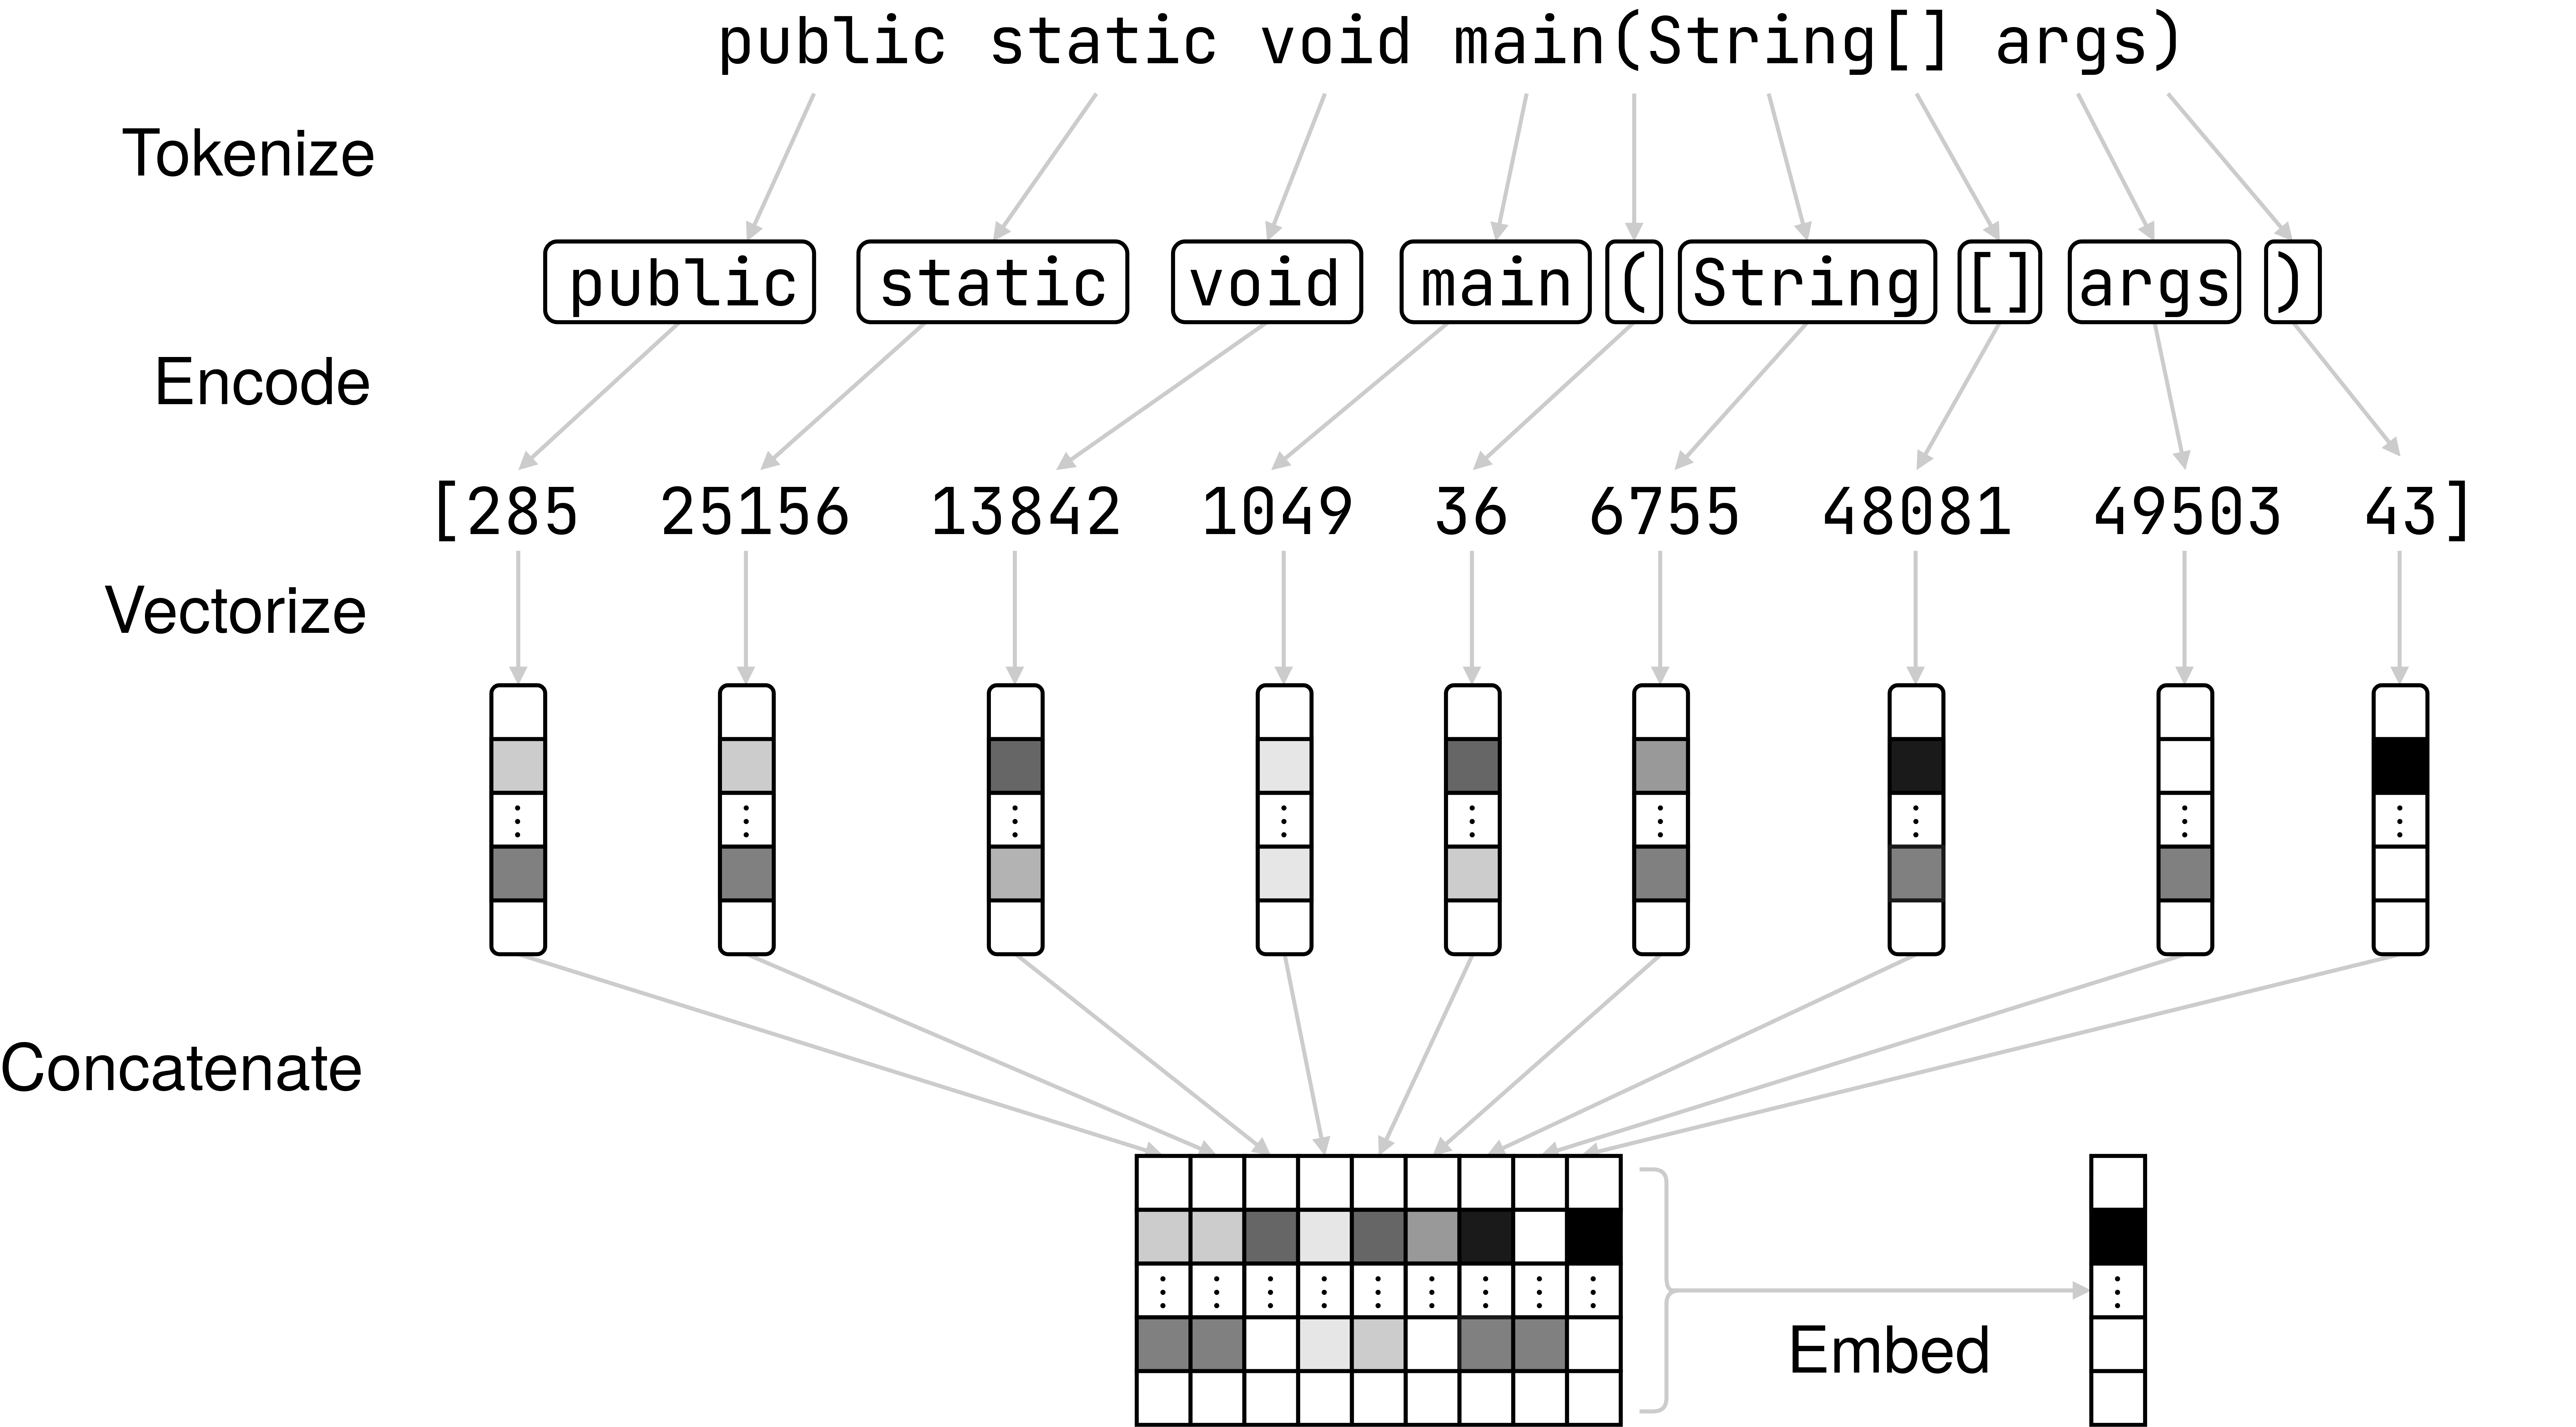
\includegraphics[width=0.40\textwidth]{figs/bert_embedding}
%     \caption{CodeBERT takes a unicode sequence and emits a vector sequence, which we accumulate into a single vector.}
%     \label{fig:bert}
%   \end{figure}

%  For each token in a string, CodeBERT emits a length-768 vector, so a line with $n$ tokens produces a matrix of shape $\mathbb R^{768 \times (n + 1)}$, the first column of which contains the final hidden layer activations. We concatenate the CodeBERT sequence `\texttt{<s>}' and using the source tokens, encode and vectorize the encoded sequence using the vocabulary, then take the first row as our sequence embedding as depicted in Fig.~\ref{fig:bert}. In \S~\ref{sec:results}, we compare various distance-metrics to fetch the nearest sequence embeddings in our database and compare precision and recall across various types of distance metrics.
%
%  \begin{figure}[H]
%    \centering
%    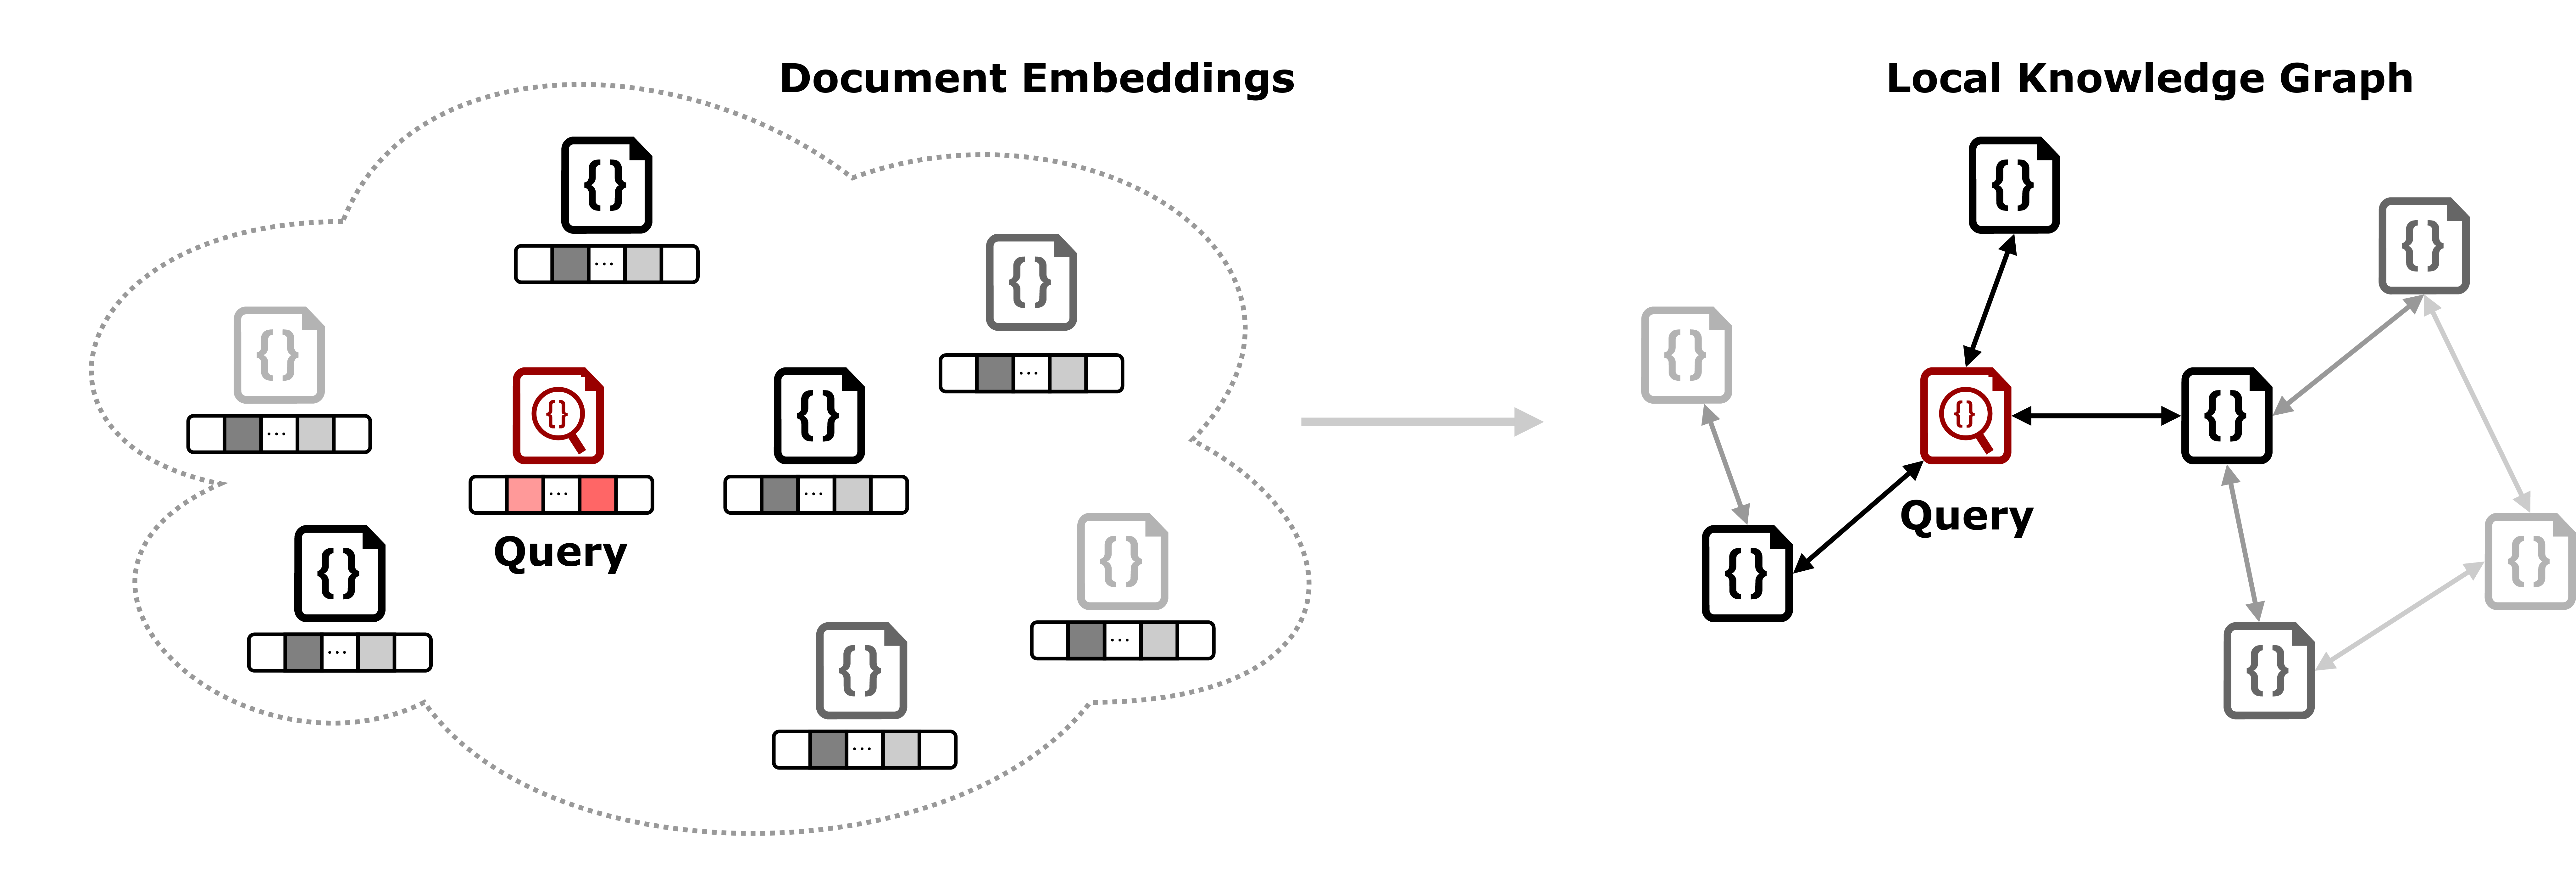
\includegraphics[width=0.4\textwidth]{figs/latent_kg}
%    \caption{To compute our query neighborhood, we traverse the HNSWG up to max depth $d$, i.e. $d=1$ fetches the neighbors, $d=2$ fetches the neighbors-of-neighbors, and $d=3$ fetches the neighbors-of-neighbors-of-neighbors.}
%    \label{fig:de2kg}
%  \end{figure}
%
%  For a given query and context, we first compute the context embedding and using a distance metric, fetch the k-nearest neighboring documents in latent space, forming the depth-1 nodes in our graph, then repeat this procedure recursively, pruning with a beam search heuristic based on the total path length in latent space. This procedure is depicted in Fig.~\ref{fig:de2kg}.
%
%  \begin{figure}[H]
%    \centering
%    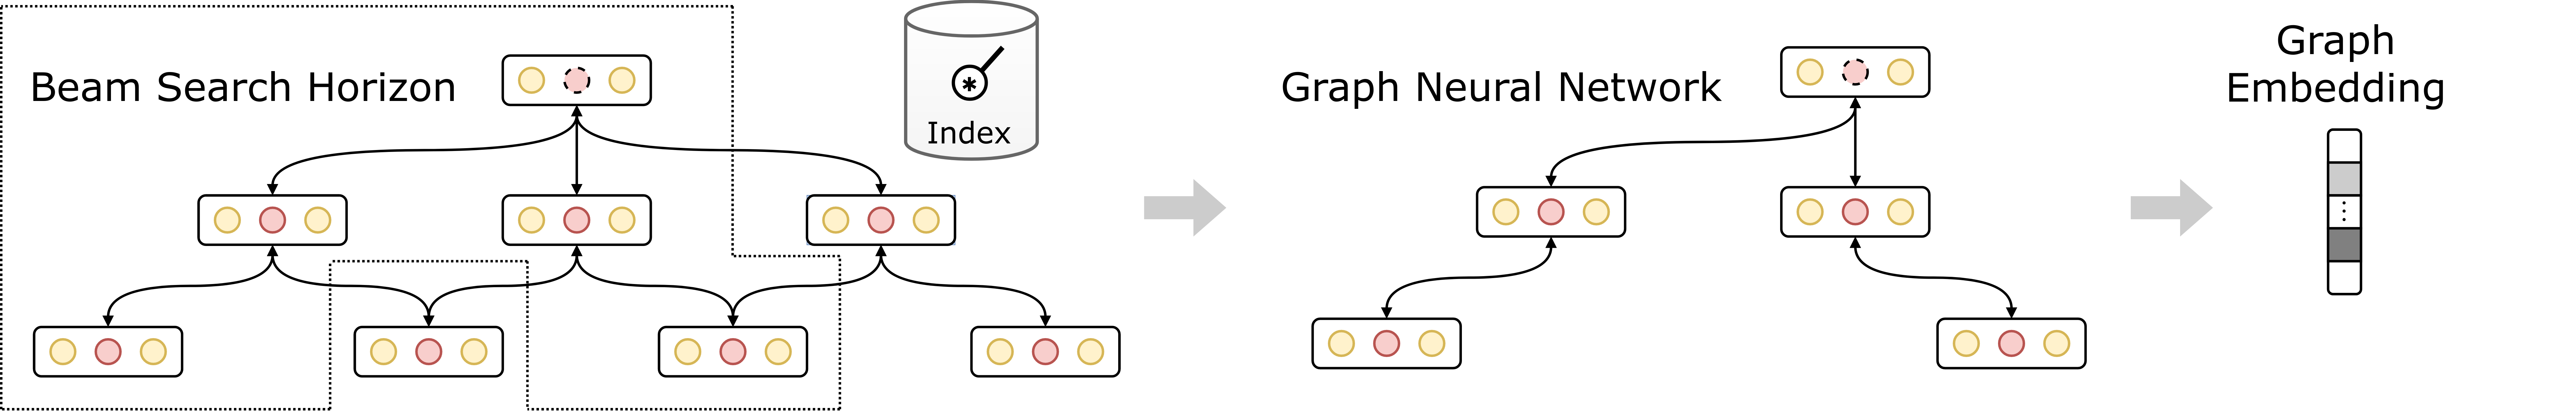
\includegraphics[width=0.4\textwidth]{figs/architecture}
%    \caption{Unlike language models which directly learn the data distribution, our model is designed to query an unseen database only available at test time. The model scores and selectively expands a subset of promising results within the database using a beam search heuristic, then runs message passing over the resulting graph to obtain the final task prediction.}
%    \label{fig:architecture}
%  \end{figure}
%
%  Consider the depth-1 beam search procedure (Fig. ~\ref{fig:pipeline}): We can use either vector search or keyword search to perform the context expansion, although vector search has the disadvantage of needing to rebuild the vector embedding index at each step during training. Keyword search is comparatively cheaper, as it only needs to build once for each repo on MiniGithub.
%
%  \begin{figure}[H]
%    \centering
%    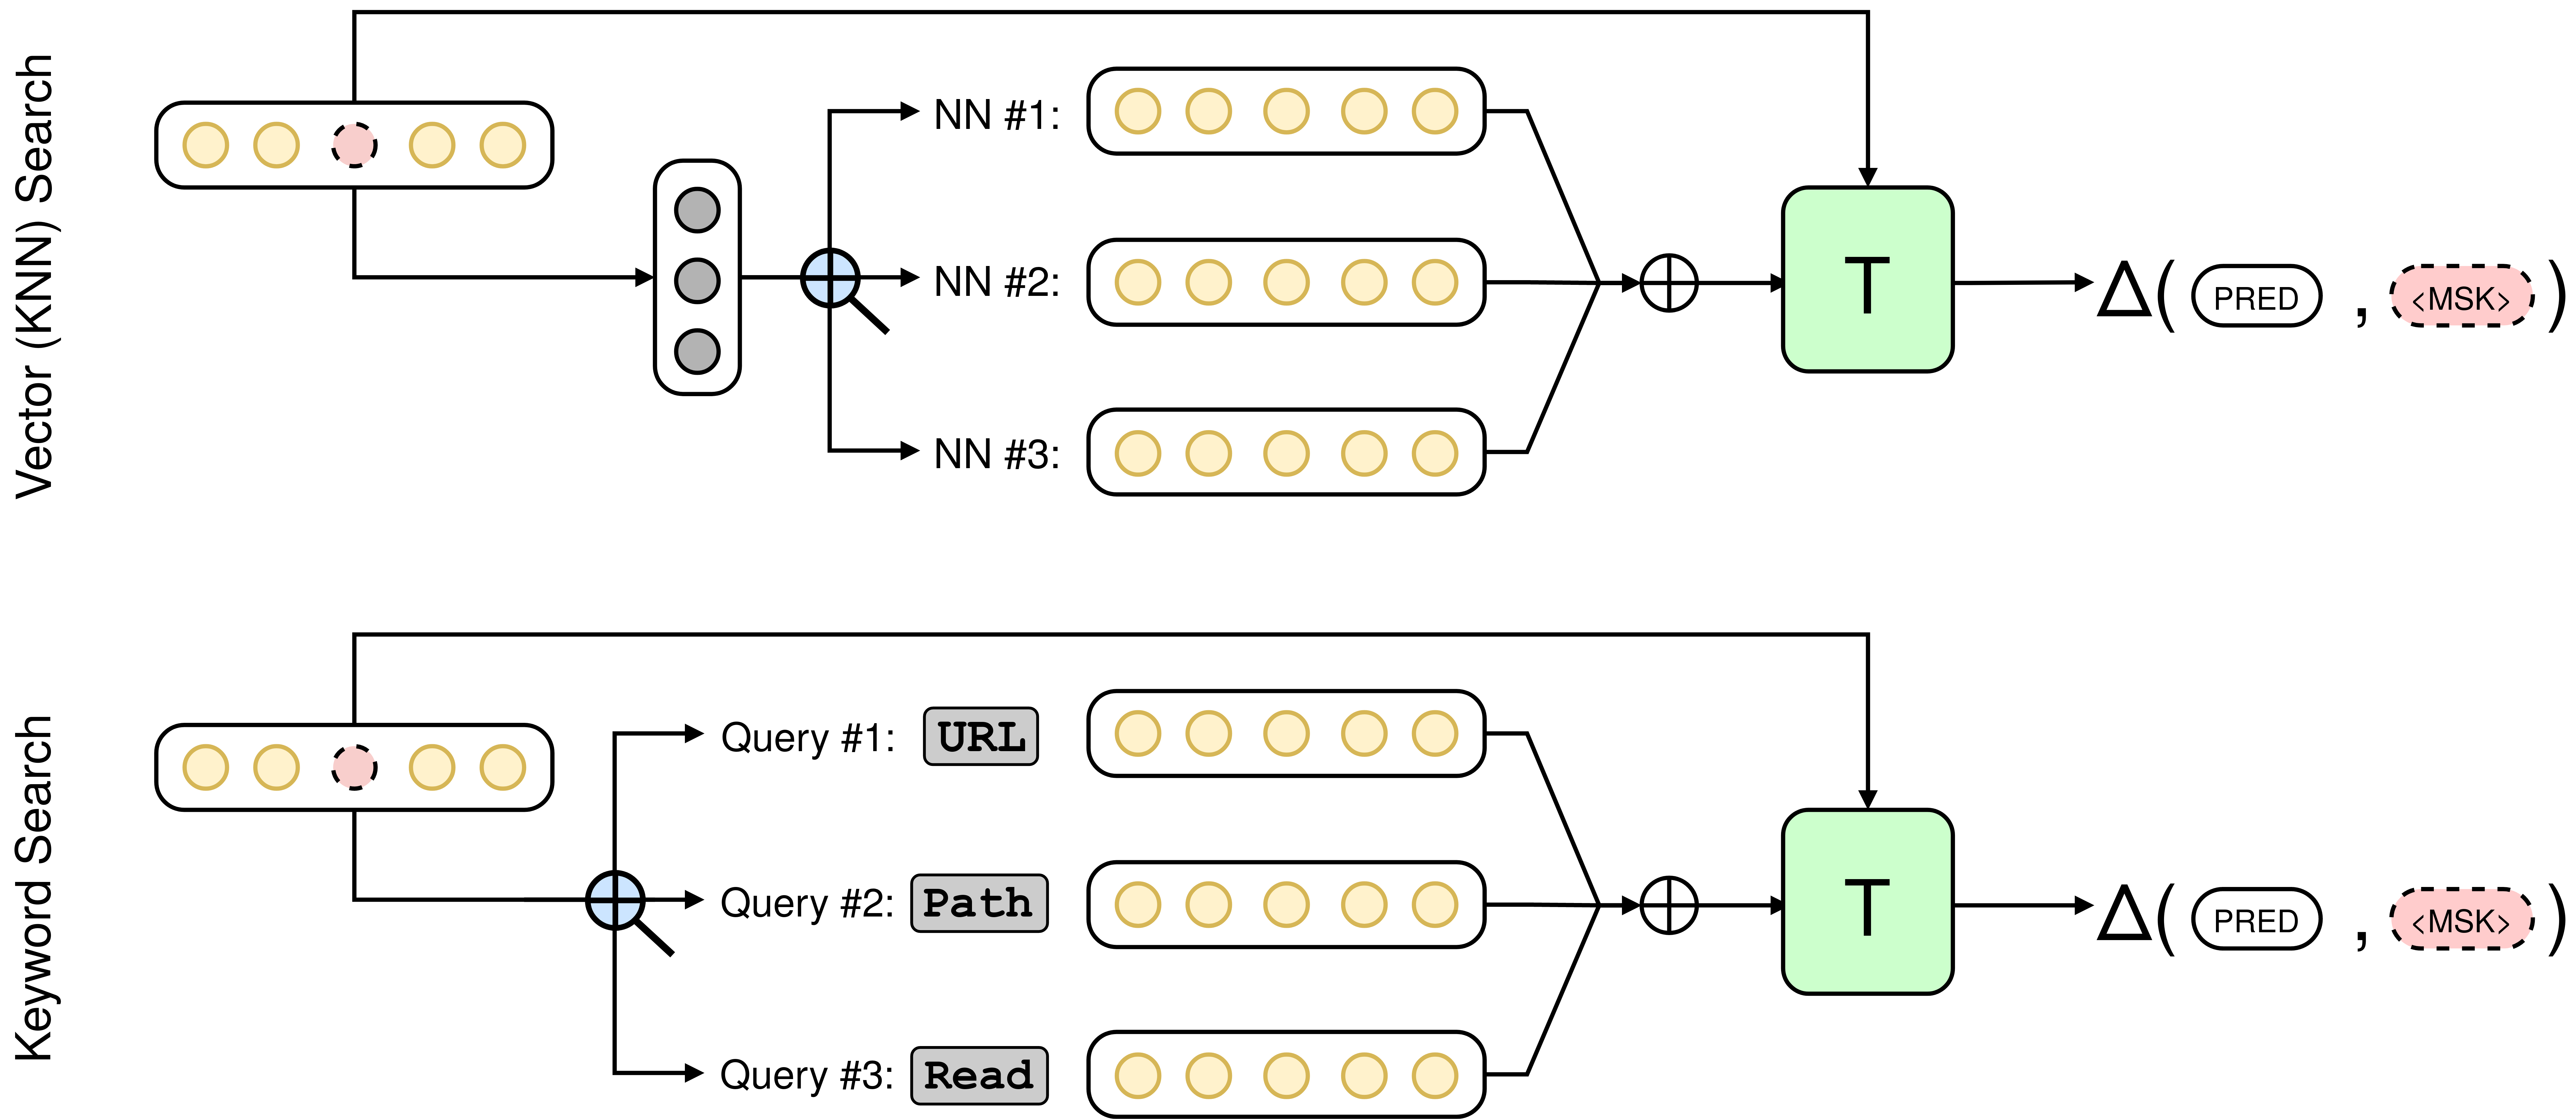
\includegraphics[width=0.4\textwidth]{figs/knn_vs_vec}
%    \caption{In the vector search procedure, we compute an embedding for the masked source context, then retrieve the k-nearest sequence embeddings in our database. In the keyword search, we compute an n-hot vector to select the keywords, and retrieve the nearest matching sequences in our index. In both cases, we embed the results, feed them into a transformer, compute a loss between the predicted output and the masked token, and backpropagate.}
%    \label{fig:pipeline}
%  \end{figure}
%
%  Once the beam search procedure is complete, we have a graph representing the neighborhood of the nearest neighboring code fragments in the parent project. This forms a so-called \textit{virtual knowledge graph}, with nodes decorated by the CodeBERT sequence embeddings and edges decorated with the direction vector between documents. We then run $p$ rounds of message passing to obtain graph embedding or \textit{neighborhood summary vector} (Fig.~\ref{fig:architecture}).

% We initialize the policy network using a pretrained language model. Starting at the site of the prediction task and conditioning on its local context, the policy network draws K queries from its latent state, which are fed into the index to produce a set of matching locations. The model scores and selectively expands a subset of those locations, and the process is repeated using finite-horizon MCTS or similar beam search procedure to retrieve a set of contextually relevant locations within the parent project.
%
%The rollout traces form a graph of related locations inside each project and their corresponding context embeddings, which together form the GNN node features. Once the rollout ends, we run message passing on the resulting GNN for a fixed numbers of steps and decode the graph embedding to obtain a task prediction. The decoder, GNN parameters, and policy network are all trained end-to-end on the downstream task, e.g. code completion, defect detection or correction. After convergence, we compare the results across horizon size and analyze the queries and filetypes which are selected.

  \pagebreak
  \section{Experiments}\label{sec:experiments}

  In this work, we attempt to understand the relationship between entities in a software project. Our research seeks to answer the following questions:

  \begin{enumerate}
    \item Which contexts in a software project share mutual information?
    \item To what degree can we claim the model has learned to:\begin{enumerate}
                                                                 \item Locate contextually relevant artifacts within a software project?
%   \item Comprehend the semantic content of the artifacts traversed?
%   \item Apply the knowledge gathered to perform the assigned task?
    \end{enumerate}
  \end{enumerate}

  {
    \renewcommand{\arraystretch}{1.5}
    \begin{table}[H]
      \small
      \begin{tabular}{l|ccc}
        Model & IRA & QDL & P/R \\
        \hline
        \href{https://huggingface.co/microsoft/CodeGPT-small-java}{\textsc{CodeGPT}}~\citep{lu2021codexglue} & X & X & X \\
        \href{https://huggingface.co/microsoft/graphcodebert-base}{\textsc{GraphCodeBERT}}~\citep{guo2021graphcodebert} & X & X & X \\
        \href{https://huggingface.co/huggingface/CodeBERTa-small-v1a}{\textsc{CodeBERT-small}}~\citep{feng2020codebert} & X & X & X \\
        \href{https://huggingface.co/dbernsohn/roberta-java}{\textsc{RoBERTa-Java}}~\citep{liu2019roberta} & X & X & X \\
        \href{https://copilot.github.com/}{\textsc{Copilot}}\citep{chen2021evaluating} & X & X & X \\

      \end{tabular}
      \caption{\label{tab:ad_comparison} Experiments table for comparing pretrained LM embeddings on source code snippets. IRA: Iterrater agreement. QDL: query description length, P/R: Precision/recall}
    \end{table}
  }


  For each of these models (available on HuggingFace), we sample a set of code snippets from our synthetic dataset, and compare how well they agree on each task.


  In contrast with classical code completion models which only require a file-local context, our method is designed to navigate an entire project. In the following experiments, we compare completion accuracy with a vanilla sequence prediction model, as well as an AST-structured sequence prediction model trained from a corpus of Java projects on the same task.

  We hypothesize that by jointly learning to choose locations in a project over which to attend while solving a downstream task, such as masked sequence completion, our model will produce a feature representation capable of locating and extracting information from semantically relevant contexts. We evaluate our hypothesis both qualitatively and quantitatively.

  In our first set of experiments, we try to understand what is shared between sequences mapped to similar latent vectors. Do similar sequences share salient keywords? Are those keywords relevant to the task?

  In our second experiment, we try to measure the information gain from including and excluding various filetypes through ablation. For graphs containing filetypes which include Markdown or Java, what kinds of information do these resources provide and which categories are most salient?

%In our third experiment, we compare prediction accuracy across architectures and datasets. Can we constrain the action space (e.g. only querying tokens from the surrounding context) for more efficient trajectory sampling, or allow arbitrary queries? How well does the model architecture transfer to new repositories, within and across programming languages?

  In our third and final set of experiments, we compare performance across hyperparameters. Does contextual expansion lead to better task performance for a given sequence prediction task? By relaxing edge-construction criteria and increasing hyperparamers such as beam search budget, we would expect corresponding task performance to increase.

  If our hypothesis is correct, the virtual knowledge graph will span both natural language and source code artifacts. If so, this would provide evidence to support the broader hypothesis~\citep{guo2017semantically} that documentation is a useful source of information. In addition to being useful for the prediction task itself, we anticipate our model could also be used for knowledge graph extraction and suggest semantically relevant code snippets to developers.



  \pagebreak
  \section{Evaluation}\label{sec:evaluation}

  \bibliography{main}
  \bibliographystyle{plain}
  \pagebreak
  \appendix

  \section{Slicing procedure}

  We describe below a simple heuristic for extracting method slices in well-formed source code using a Dyck counter. A common coding convention is to prefix functions with a keyword, followed by a group of balanced brackets and one or more blank lines. While imperfect, we observe this pattern can be used to slice methods in a variety of langauges in practice. A Kotlin implementation is given below, which will output the following source code when run on itself:

  \vspace{11pt}

  \begin{lstlisting}[basicstyle=\scriptsize\ttfamily, language=kotlin,label={lst:lstlisting}]
fun String.sliceIntoMethods(kwds: Set<String> = setOf("fun ")) =
  lines().fold(-1 to List<String>(0)) { (dyckCtr, methods), ln ->
    if (dyckCtr < 0 && kwds.any { it in ln }) {
      ln.countBalancedBrackets() to (methods + ln)
    } else if (dyckCtr == 0) {
      if (ln.isBlank()) -1 to methods else 0 to methods.put(ln)
    } else if (dyckCtr > 0) {
      dyckCtr + ln.countBalancedBrackets() to methods.put(ln)
    } else -1 to methods
  }.second

fun List<String>.put(s: String) = dropLast(1) + (last() + "\n$s")

fun String.countBalancedBrackets() = fold(0) { sum, char ->
  val (lbs, rbs) = setOf('(', '{', '[') to setOf(')', '}', ']')
  if (char in lbs) sum + 1 else if (char in rbs) sum - 1 else sum
}

fun main(args: Array<String>) =
  println(args[0].sliceIntoMethods().joinToString("\n\n"))
  \end{lstlisting}

  \section{Analysis of internal structure}

  Our preliminary results compare distance metrics (Fig.~\ref{fig:lev_vs_euclid}), explore embedding quality (Fig.~\ref{fig:embedding}) and visualize the synthetic knowledge graphs (Fig.~\ref{fig:graphs}).

  \begin{figure}[H]
    \centering
    \resizebox{0.45\textwidth}{!}{%
      \begin{tikzpicture}
        \begin{axis}[width=0.29\textwidth, height=0.3\textwidth, ymax=7, xlabel=Levenshtein, ylabel=Euclidean]
          \addplot table [mark=none,x=strdist, y=embdist, variable=var, col sep=comma] {data/levenshtein.csv};

          \addplot [smooth, name path=upper,draw=none] table[x=strdist, y=embdist,variable=var, y expr=\thisrow{embdist}+\thisrow{var}, col sep=comma] {data/levenshtein.csv};
          \addplot [smooth, name path=lower,draw=none] table[x=strdist, y=embdist,variable=var, y expr=\thisrow{embdist}-\thisrow{var}, col sep=comma] {data/levenshtein.csv};
          \addplot [fill=red!10] fill between[of=upper and lower];
        \end{axis}
      \end{tikzpicture}
      \begin{tikzpicture}
        \begin{axis}[width=0.29\textwidth, height=0.3\textwidth, ymax=7, xlabel=Damerau]
          \addplot table [mark=none,x=strdist, y=embdist, variable=var, col sep=comma] {data/damerau.csv};

          \addplot [smooth, name path=upper,draw=none] table[x=strdist, y=embdist,variable=var, y expr=\thisrow{embdist}+\thisrow{var}, col sep=comma] {data/damerau.csv};
          \addplot [smooth, name path=lower,draw=none] table[x=strdist, y=embdist,variable=var, y expr=\thisrow{embdist}-\thisrow{var}, col sep=comma] {data/damerau.csv};
          \addplot [fill=red!10] fill between[of=upper and lower];
        \end{axis}
      \end{tikzpicture}
      \begin{tikzpicture}
        \begin{axis}[width=0.29\textwidth, height=0.3\textwidth, ymax=7, xlabel=MetricLCS]
          \addplot table [mark=none,x=strdist, y=embdist, variable=var, col sep=comma] {data/metriclcs.csv};

          \addplot [smooth, name path=upper,draw=none] table[x=strdist, y=embdist,variable=var, y expr=\thisrow{embdist}+\thisrow{var}, col sep=comma] {data/metriclcs.csv};
          \addplot [smooth, name path=lower,draw=none] table[x=strdist, y=embdist,variable=var, y expr=\thisrow{embdist}-\thisrow{var}, col sep=comma] {data/metriclcs.csv};
          \addplot [fill=red!10] fill between[of=upper and lower];
        \end{axis}
      \end{tikzpicture}
      \begin{tikzpicture}
        \begin{axis}[width=0.29\textwidth, height=0.3\textwidth, ymax=7, xlabel=Jaccard]
          \addplot table [mark=none,x=strdist, y=embdist, variable=var, col sep=comma] {data/jaccard.csv};

          \addplot [smooth, name path=upper,draw=none] table[x=strdist, y=embdist,variable=var, y expr=\thisrow{embdist}+\thisrow{var}, col sep=comma] {data/jaccard.csv};
          \addplot [smooth, name path=lower,draw=none] table[x=strdist, y=embdist,variable=var, y expr=\thisrow{embdist}-\thisrow{var}, col sep=comma] {data/jaccard.csv};
          \addplot [fill=red!10] fill between[of=upper and lower];
        \end{axis}
      \end{tikzpicture}
    }
    \caption{CodeBERT latent space distance correlates with string edit distance.}
    \label{fig:lev_vs_euclid}
  \end{figure}

  \begin{figure}[H]
    \centering
    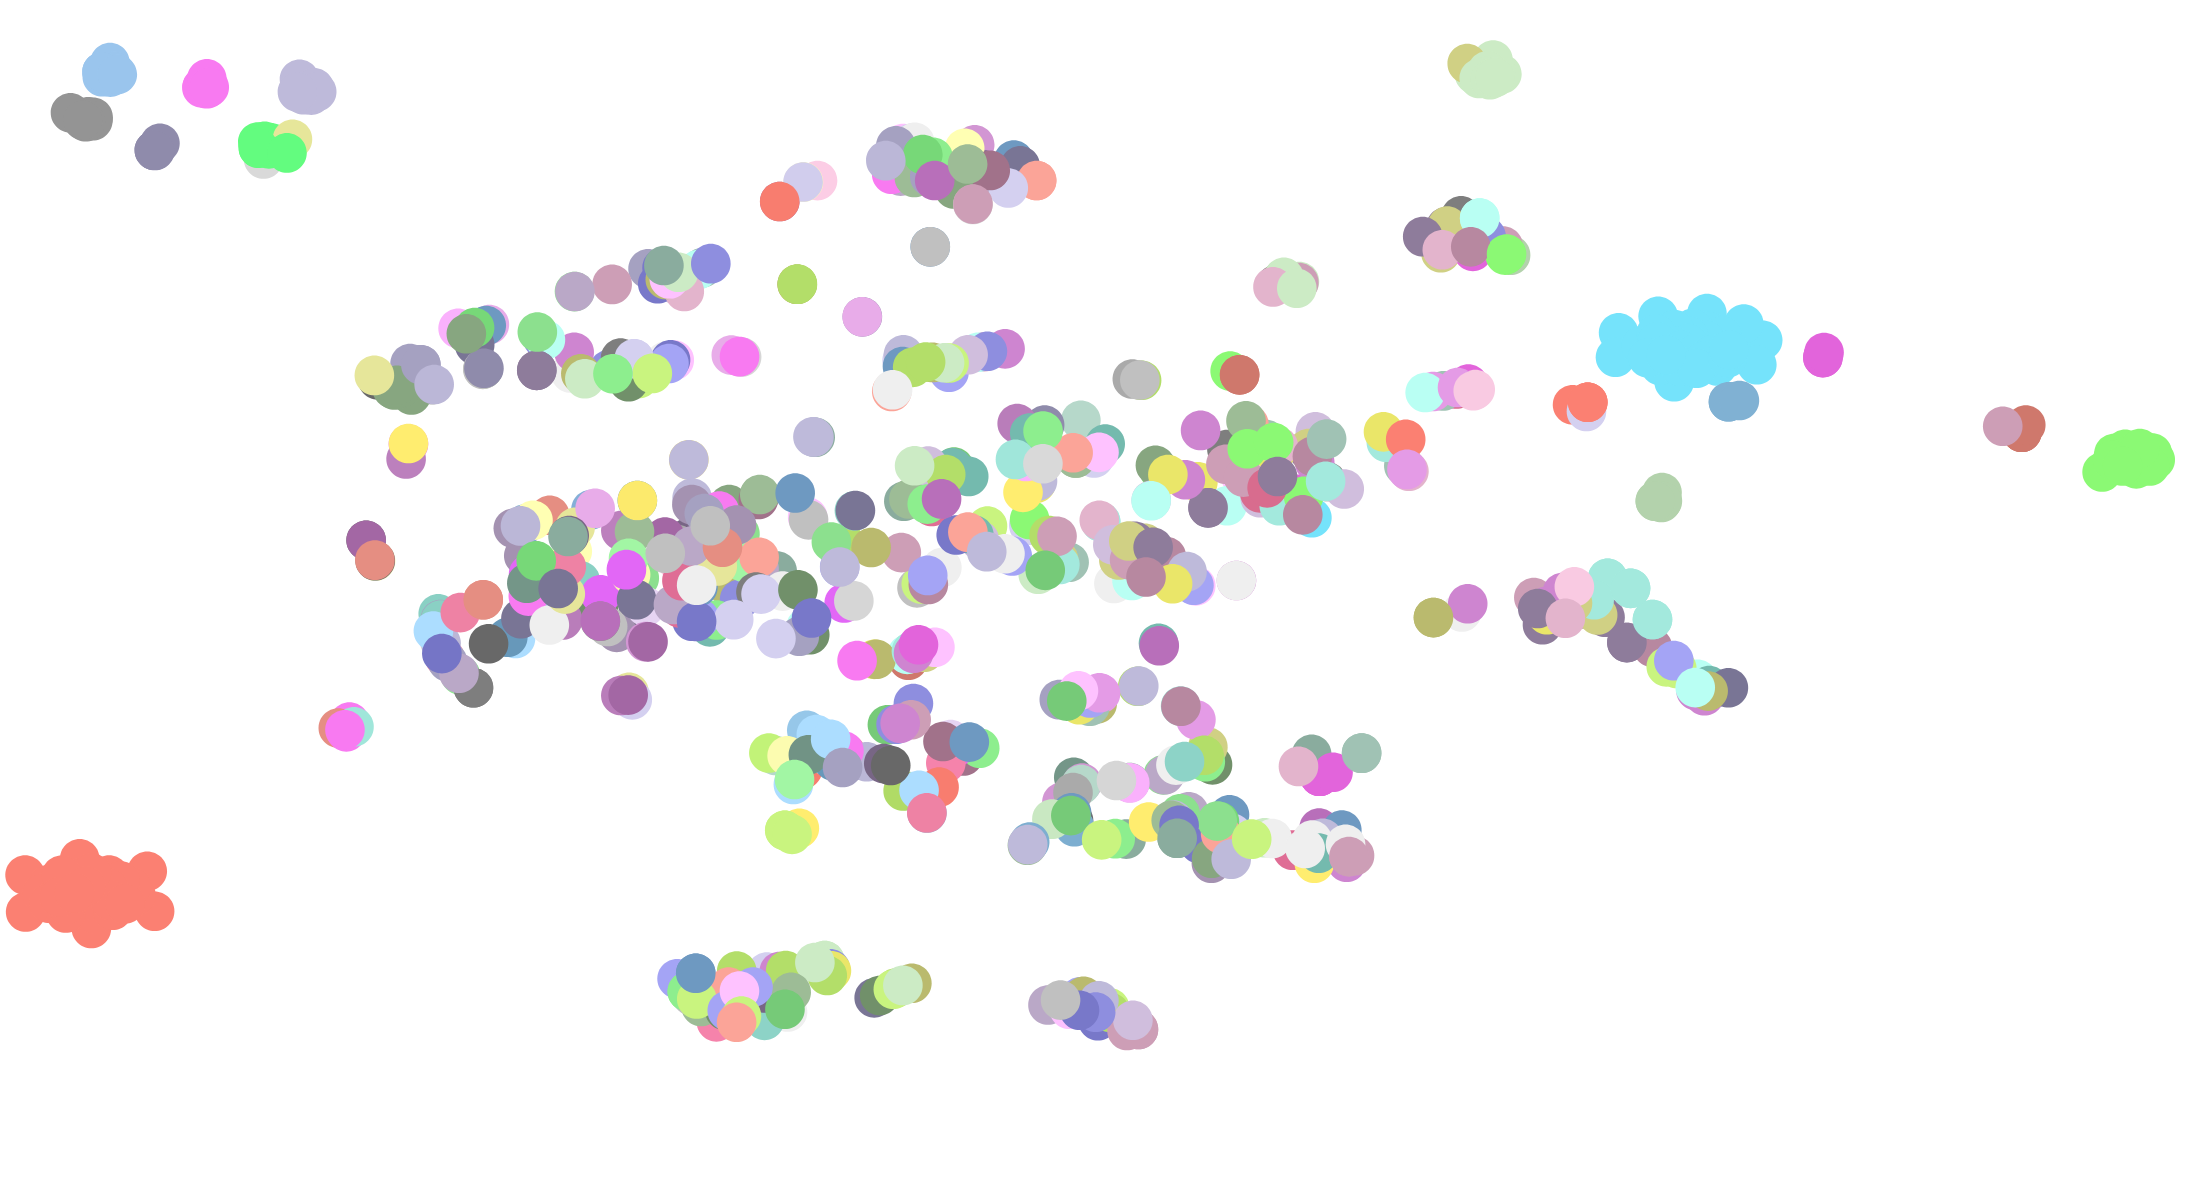
\includegraphics[width=0.4\textwidth]{figs/embeddings}
    \caption{Reduced dimensionality TNSE embeddings colored by line length.}
    \label{fig:embedding}
  \end{figure}

  \begin{figure}[H]
    \centering
    \resizebox{.1\textwidth}{!}{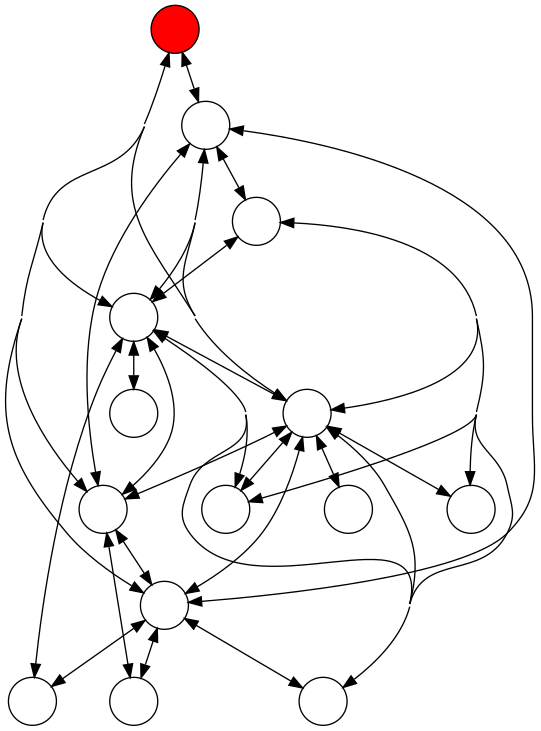
\includegraphics{../data/query4}}
    \resizebox{.1\textwidth}{!}{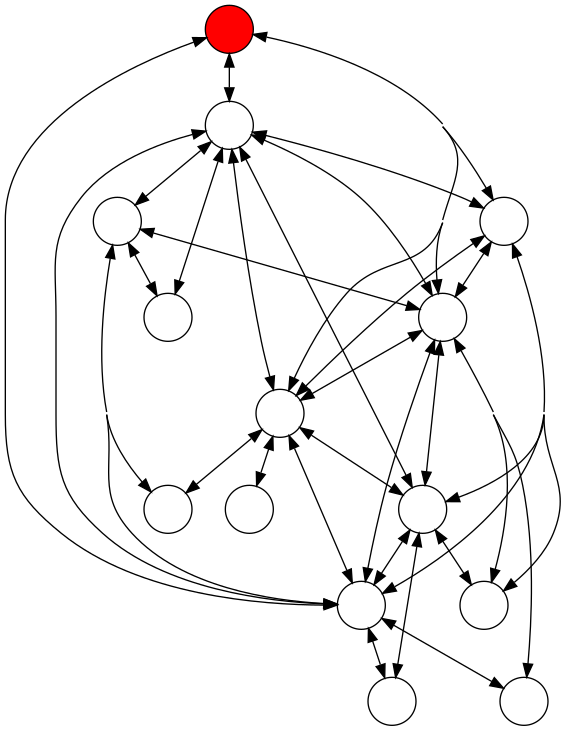
\includegraphics{../data/query5}}
    \resizebox{.1\textwidth}{!}{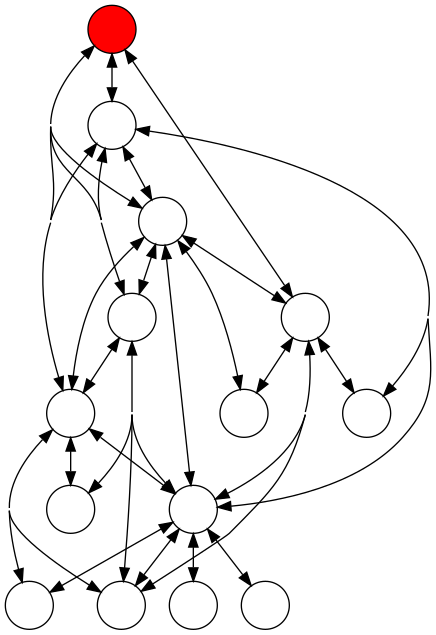
\includegraphics{../data/query6}}
    \resizebox{.1\textwidth}{!}{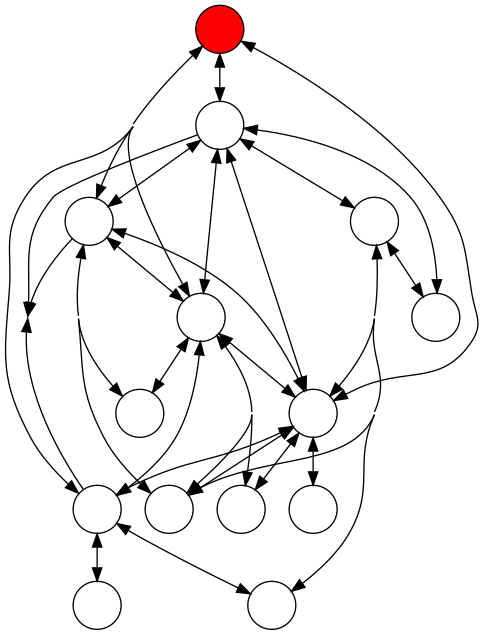
\includegraphics{../data/query7}}
    \resizebox{.1\textwidth}{!}{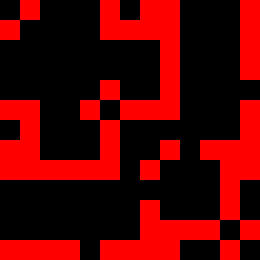
\includegraphics{../data/context4}}
    \resizebox{.1\textwidth}{!}{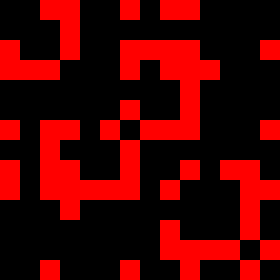
\includegraphics{../data/context5}}
    \resizebox{.1\textwidth}{!}{
\includegraphics{../data/context6}}
    \resizebox{.1\textwidth}{!}{
\includegraphics{../data/context7}}
    \caption{Virtual knowledge graph constructed by visiting nearest-neighbors in latent space.}
    \label{fig:graphs}
  \end{figure}


\end{document}
\endinput